% !TeX root = ../tesis.tex


\section{Secciones transversales}
\label{section:yth}
La interacción luz–materia puede describirse clásicamente mediante dos procesos fundamentales: la absorción y el esparcimiento, cuyo efecto conjunto se denomina extinción \cite{bohrenAbsorptionScatteringLight2008}. Experimentalmente, estos fenómenos se evidencian al comparar la potencia medida por un detector con y sin la presencia de una partícula iluminada por un campo electromagnético incidente  ($\vb{E}_{\text{inc}}, \vb{H}_{\text{inc}}$) la cual genera un campo electromagnético esparcido ($\vb{E}_{\text{sca}}, \vb{H}_{\text{sca}}$) como se ejemplifica en la Fig. \ref{scattering}, donde se muestra una partícula arbitraria sobre la cual incide un campo electromagnético ($\vb{E}_{\text{inc}}, \vb{H}_{\text{inc}}$), produciendo el campo electromagnético esparcido ($\vb{E}_{\text{sca}}, \vb{H}_{\text{sca}}$) ~\cite{bohrenAbsorptionScatteringLight2008}.
%
\begin{figure}[t]
	\centering
	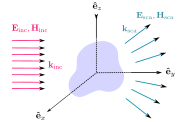
\includegraphics[width=8.5cm]{../../Figuras/scattering.pdf}
	\caption{Diagrama del problema de esparcimiento. El campo electromagnético ($\vb{E}_{\text{inc}}, \vb{H}_{\text{inc}}$) incide sobre una partícula arbitraria, produciendo el campo electromagnético esparcido ($\vb{E}_{\text{sca}}, \vb{H}_{\text{sca}}$).}
	\label{scattering}
\end{figure}
%

Para cuantificar este efecto de manera macroscópica, en esta sección se introducen las secciones transversales de extinción, absorción y esparcimiento, al considerar a la partícula embebida en un medio no absorbente e iluminada por una onda plana~\cite{bohrenAbsorptionScatteringLight2008}. Bajo estas condiciones, la energía transportada por los campos electromagnéticos que es absorbida por la partícula $W_{\text{abs}}$, se calcula al integrar el promedio temporal del vector de Poynting  $\langle\vb{S}\rangle_t$  sobre una superficie cerrada $A$, lo suficientemente grande para encontrarse en el régimen de campo lejano. Para simplificar el análisis, dicha superficie se toma como una esfera de radio $r$ que encierra completamente a la partícula, como se muestra en la Fig. \ref{WA}, es decir, 
\begin{tcolorbox}[ams align]
	W_{\text{abs}}=-\int_A \langle\vb{S}\rangle_t\cdot\vu{e}_r \text{ dA},
	\label{flujopoynting}
\end{tcolorbox}
\noindent donde $\langle\vb{S}\rangle_t$ y $\vu{e}_r$ son paralelos y el signo negativo garantiza que $W_{\text{abs}}$ sea una cantidad positiva definida, asumiendo que únicamente hay procesos de absorción y no de emisión \cite{bohrenAbsorptionScatteringLight2008}.
%
\begin{figure}[b]
	\centering
	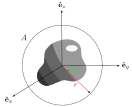
\includegraphics[width=7cm]{../../Figuras/WA.pdf}
	\caption{Esquema de la superficie de integración $A$ como una esfera de radio $r$ centrada en el origen y que encierra a una partícula.}
	\label{WA}
\end{figure}
%
\noindent Es posible descomponer el vector de Poynting total en tres contribuciones \cite{bohrenAbsorptionScatteringLight2008}
%		
\begin{subequations}%
	\begin{tcolorbox}[
		ams align, breakable]
\langle\vb{S}_{\text{inc}}\rangle_t&=  \frac{1}{2}\:\mbox{Re}\{\vb{E}_{\text{inc}}\times\vb{H}_\text{inc}^*\},\\%
	\langle\vb{S}_{\text{sca}}\rangle_t&=  \frac{1}{2}\:\mbox{Re}\{\vb{E}_{\text{sca}}\times\vb{H}_{\text{sca}}^*\},\\%
	\langle\vb{S}_{\text{ext}}\rangle_t&= \frac{1}{2}\:\mbox{Re}\{\vb{E}_{\text{inc}}\times\vb{H}_{\text{sca}}^*+\vb{E}_{\text{sca}}\times\vb{H}_\text{inc}^*\},\label{eq:S}%
\end{tcolorbox}
\end{subequations}
%
\noindent donde los subíndices \enquote*{inc}, \enquote*{sca} y \enquote*{ext} se refieren al campo incidente, al campo esparcido y a la interacción entre los dos anteriores, respectivamente, se obtiene al integrar que $W_{\text{abs}}=~W_{\text{inc}}-~W_{\text{sca}}+~W_{\text{ext}}$, donde \cite{bohrenAbsorptionScatteringLight2008}
%
\begin{subequations}\label{eqs:W}
	\begin{align} 
		W_{\text{inc}}  &= -\int_{A}\langle\vb{S}_{\text{inc}}\rangle_t\cdot\vu{e}_r\text{ dA}, \label{seq:Wi}\\
		W_{\text{sca}} &= \int_{A}\langle\vb{S}_{\text{sca}}\rangle_t\cdot\vu{e}_r\text{ dA}, \label{seq:Ws} \\ 
		W_{\text{ext}} &= -\int_{A}\langle\vb{S}_{\text{ext}}\rangle_t\cdot\vu{e}_r\text{ dA}. \label{seq:Wext}
	\end{align}
\end{subequations}
%
Los signos de las Ecs. \eqref{eqs:W} se eligen de forma que sean cantidades positivas considerando las direcciones de los vectores de Poynting y de $\vu{e}_r$. Como la energía del campo incidente que cruza la esfera es la misma que la que entra, $W_{\text{inc}}$ se anula, entonces
%
\begin{equation}
	W_{\text{ext}}=W_{\text{abs}}+W_{\text{sca}}.
	\label{Wext_tot}
\end{equation}
%%

Asumiendo que la contribución dominante del campo esparcido es la dipolar, una partícula iluminada por una onda plana $\vb{E}_{\text{inc}} = E_0\,\vu{e}_x$, con $\vb{H}_{\text{inc}} = (k/\mu\omega)\,\vu{e}_z\times\vb{E}_{\text{inc}}$, puede describirse mediante un momento dipolar inducido $\vb{p}$ caracterizado por una polarizabilidad $\alpha$. Por lo tanto, el campo esparcido se describe como una onda esférica de frecuencia angular $\omega$ dada por \cite{bohrenAbsorptionScatteringLight2008}
%
\begin{align}
	\vb{E}_{\text{sca}}&=\frac{e^{ik(r-z)}}{-ikr}\vb{X}\:E_0 \qquad\text{y}\qquad
	\vb{H}_{\text{sca}}=\frac{k}{\omega\mu}\vu{e}_r\times\vb{E}_{\text{sca}},
	\label{eq:EH_s}
\end{align}
%
donde $\vb{X}$ es el vector de amplitud de esparcimiento
%
\begin{equation}
	\vb{X}=\frac{ik^3}{4\pi}\alpha \left[ \vu{e}_r\times(\vu{e}_r\times \vu{e}_x)\right].
	\label{eq:Xvec}
\end{equation}
%
A partir de las Ecs.~\eqref{eq:EH_s} y de las ecuaciones del campo electromagnético incidente ($\vb{E}_{\text{inc}} , \vb{H}_{\text{inc}} $), es posible determinar $W_{\text{ext}}$, que se obtiene a partir de $\langle\vb{S}_{\text{ext}}\rangle_t$, definido en la Ec.~\eqref{eq:S}. Para ello se considera\footnote{En donde de empleó la identidad del triple producto vectorial dada por $\vb{A}\times(\vb{B}\times\vb{C})=\vb{B}(\vb{A}\cdot\vb{C})-\vb{C}(\vb{A}\cdot\vb{B})$~\cite{griffithsIntroductionElectrodynamics2023b}.}
%
\begin{align*}
	\vb{E}_{\text{inc}}\times\vb{H}_{\text{sca}}^*&=E_0\vu{e}_x\times\left(\frac{k}{\omega\mu}\vu{e}_r\times \vb{E}_{\text{sca}}\right)^*\\
	&=\frac{k|E_0|^2}{\omega\mu}\frac{e^{-ik(r-z)}}{ikr}[\vu{e}_r(\vu{e}_x\cdot\vb{X}^*)-\vb{X}^*(\vu{e}_x\cdot\vu{e}_r)],
\end{align*}
%
y análogamente,
%
\begin{equation*}
	\vb{E}_{\text{sca}}\times\vb{H}_{\text{inc}}^*=\frac{k|E_0|^2}{\omega\mu}\frac{1}{-ikr}[\vu{e}_z(\vb{X}\cdot\vu{e}_x)-\vu{e}_x(\vb{X}\cdot\vu{e}_z)].
\end{equation*}
%
De esta forma,
%
\begin{align}
	\langle\vb{S}_{\text{ext}}\rangle_t=\frac{1}{2}\:\mbox{Re}&\biggl\{\frac{k|E_0|^2}{\omega\mu}\frac{e^{-ik(r-z)}}{ikr}[\vu{e}_r(\vu{e}_x\cdot\vb{X}^*)-\vb{X}^*(\vu{e}_x\cdot\vu{e}_r)]+ \nonumber\\ 
	&+\frac{k|E_0|^2}{\omega\mu}\frac{1}{-ikr}[\vu{e}_z(\vb{X}\cdot\vu{e}_x)-\vu{e}_x(\vb{X}\cdot\vu{e}_z)]\biggl\}.\label{eq:S_1}
\end{align}
%
Sustituyendo la Ec. \eqref{eq:S_1} en la Ec. \eqref{seq:Wext} y empleando las relaciones $\vb{X}\cdot \vu{e}_r=~0, \vu{e}_r\cdot~\vu{e}_z=~\cos\theta$ y $\vu{e}_r\cdot~\vu{e}_x=\cos\varphi\sin\theta$, se obtiene
%
\begin{align}
		W_{\text{ext}} = -\int_{A}\langle\vb{S}_{\text{ext}}\rangle_t\cdot\vu{e}_r\text{ dA}&=\frac{|E_0|^2k}{\omega\mu}\text{Re}\biggl\{\frac{e^{-ikr}}{ikr}\int_A e^{ikz}\left(\vu{e}_x\cdot\vb{X}^*\right)\dd{a}+ \nonumber\\
		& +\frac{e^{-ikr}}{ikr}\int_A e^{-ikz}\left(\vb{X}\cdot\vu{e}_x\right)\cos\theta\dd{a}+\nonumber\\
		&-\frac{e^{-ikr}}{ikr}\int_Ae^{-ikz}\left(\vb{X}\cdot\vu{e}_z\right)\sin\theta\cos\varphi \dd{a}, \label{eq:Wext_0}
\end{align}
%
que al integrar por partes\footnote{La Ec. \eqref{eq:Wext_0} presenta integrales del tipo
$$\int_{-1}^{1}e^{ikr\mu}f(\mu)\dd{\mu},$$
con $\mu=\cos\theta$, que al integrar por partes dos veces resulta en \cite{bohrenAbsorptionScatteringLight2008}
$$\int_{-1}^{1}e^{ikr\mu}f(\mu)\dd{\mu}=f(\mu)\frac{e^{ikr\mu}}{ikr}\Big|_{-1}^{1}+\frac{1}{(kr)^2}\left[\dv{f}{\mu}e^{ikr\mu}\Big|_{-1}^{1}-\int_{-1}^1\dv[2]{f}{x}\right],$$
y como $kr\ll1$, entonces \cite{bohrenAbsorptionScatteringLight2008}
$$\int_{-1}^{1}e^{ikr\mu}f(\mu)\dd{\mu}\approx \frac{1}{ikr}\left[f(1)e^{ikr}-f(-1)e^{-ikr}\right].$$ }, simplificando se tiene que \cite{bohrenAbsorptionScatteringLight2008}
%
\begin{equation*}
	W_{\text{ext}}=I_{\text{inc}}\frac{4\pi}{k^2}\:\text{Re}\{(\vb{X}\cdot\vu{e}_x)_{\theta=0}\},
\end{equation*}
%
con $I_{\text{inc}}$ la irradiancia de la onda incidente, que corresponde a la magnitud de $\langle\vb{S}_{\text{inc}}\rangle_t$, y por consiguiente\footnote{Debido al teorema óptico, la extinción sólo depende de la amplitud de esparcimiento en la dirección de propagación y es el efecto combinado de la absorción en la partícula y el esparcimiento por la partícula en todas las direcciones \cite{bohrenAbsorptionScatteringLight2008}.},
%
\begin{equation}
	C_{\text{ext}}=\frac{W_{\text{ext}}}{I_{\text{inc}}}=\frac{4\pi}{k^2}\:\text{Re}\{(\vb{X}\cdot\vu{e}_x)_{\theta=0}\}, \label{C_ext}
\end{equation}
%
que es la sección transversal de extinción y que posee dimensiones de área.
 Al sustituir las Ecs.~(\ref{eq:EH_s}) en la Ec. (\ref{seq:Ws}) se obtiene
%
\begin{equation}
	C_{\text{sca}}=\int_0^{2\pi}\int_0^{\pi}\frac{|\vb{X}|^2}{k^2}\:\sin\theta\: \text{d}\theta\:\text{d}\phi.
	\label{C_sca_general}
\end{equation}
%%

 \noindent Finalmente, la Ec. (\ref{Wext_tot}) puede ser reescrita como \cite{bohrenAbsorptionScatteringLight2008}
%
\begin{tcolorbox}[ams align]
	C_{\text{ext}}=C_{\text{abs}}+C_{\text{sca}},
	\label{C} 
\end{tcolorbox}
%
\noindent donde $C_{\text{abs}}=W_{\text{abs}}/I_{\text{inc}}$ y $C_{\text{sca}}=W_{\text{sca}}/I_{\text{inc}}$ corresponden a las secciones transversales de absorción y esparcimiento, respectivamente.
Las Ecs. (\ref{C_ext})–(\ref{C}) son propiedades macroscópicas y medibles que proveen información sobre la energía absorbida y esparcida por una partícula \cite{bohrenAbsorptionScatteringLight2008}. Existen diversos métodos experimentales para determinar la sección transversal de extinción, entre ellos la espectroscopía basada en la ley de Beer–Lambert \cite{bohrenAbsorptionScatteringLight2008} y la microscopía holográfica digital \cite{subediMeasurementExtinctionCross2014}. Ambos se fundamentan en medir la superposición entre la onda incidente y la esparcida por la partícula en la dirección de propagación.

